\section{Stack frame}
Supponiamo di aver scritto una funzione ricorsiva, cioè una funzione che chiama se stessa, e di voler usare delle variabili che esistano solo in quella chiamata e non in tutte le altre a catena.
Se usiamo variabili in memoria dichiarate tramite la direttiva BYTE esse sono comunque globali quindi non private alla singola chiamata a funzione, così lo sono anche i registri che sono globali e statici.
Non abbiamo quindi delle variabili che abbiano lo \emph{scope} della funzione.

Per ottenere ciò possiamo fare riferimento allo stack:
quando entriamo in una procedura viene inserito sullo stack il contenuto del registro IP quando stava eseguendo la CALL/RCALL, quindi è stato effettivamente modificato.
Possiamo quindi spostare in alto ancora di più SP e procurarci una zona dello stack che sia privata per questa chiamata, inseriamo le nostre variabili qua dentro, le usiamo ed una volta finita la procedura prima di eseguire la ret riportiamo SP al valore iniziale in modo da poter eseguire la ret correttamente e liberare lo stack da queste variabili temporanee.
\begin{figure}[H]
    \centering
    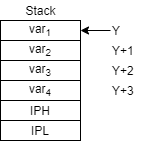
\includegraphics[width=125px]{images/20_Stack_frames/stack_frame.png}
\end{figure}
Per accedere a queste variabili allocate sullo stack viene comodo l' indirzzamento con offset del registro Y:
\begin{verbatim}
    ld r0, Y+1
\end{verbatim}

